\documentclass[12pt,letterpaper]{article}
% Content lives in metadata.tex and sections/. Compile with pdfLaTeX.
\usepackage[letterpaper,margin=1in,headheight=16pt,headsep=18pt,footskip=28pt]{geometry}
\usepackage[T1]{fontenc}
\usepackage[utf8]{inputenc}
\usepackage[scaled=1.0]{helvet}
\usepackage[table]{xcolor}
\usepackage{array,booktabs,longtable,tabularx,ragged2e}
\usepackage{enumitem,fancyhdr,lastpage,titlesec,setspace}
\usepackage[printonlyused]{acronym}
\usepackage{graphicx,caption,needspace,amsmath,amssymb,etoolbox}
\usepackage[
  backend=biber,
  style=ieee,
  sorting=none
]{biblatex}

\addbibresource{references.bib}

\usepackage{hyperref}

\definecolor{QueensBurgundy}{HTML}{9D1939}
\definecolor{SmithBlue}{HTML}{00305E}
\definecolor{LightGray}{HTML}{F1F2F4}
\definecolor{MidGray}{HTML}{D6D9DD}
\definecolor{TextGray}{HTML}{343A40}


\pdfmapfile{+pdftex35.map}
\pdfmapfile{+uhv.map}
\renewcommand{\familydefault}{\sfdefault}
\onehalfspacing
\setlength{\parindent}{0pt}
\setlength{\parskip}{6pt}
\setlength{\tabcolsep}{5pt}
\renewcommand{\arraystretch}{1.18}
\setlength{\emergencystretch}{2em}
\setlist[itemize]{leftmargin=1.45em,itemsep=2pt,topsep=3pt}
\setlist[enumerate]{leftmargin=1.75em,itemsep=2pt,topsep=3pt}
\raggedbottom
\widowpenalty=10000
\clubpenalty=10000
\setcounter{tocdepth}{2}
\setcounter{secnumdepth}{2}

\titleformat{\section}
  {\Large\bfseries\color{QueensBurgundy}\centering}
  {\thesection.}{0.5em}{}
\titleformat{\subsection}
  {\normalsize\bfseries\color{QueensBurgundy}}
  {\thesubsection}{0.6em}{}
\titleformat{\subsubsection}
  {\normalsize\bfseries\color{SmithBlue}}
  {\thesubsubsection}{0.6em}{}
\titlespacing*{\section}{0pt}{8pt}{12pt}
\titlespacing*{\subsection}{0pt}{12pt}{4pt}
\titlespacing*{\subsubsection}{0pt}{10pt}{3pt}


\newcommand{\CourseSection}[1]{\section{#1}}
\newcommand{\CourseSubsection}[1]{\subsection{#1}}
\newcommand{\UnnumberedSection}[1]{%
  \section*{#1}\phantomsection\addcontentsline{toc}{section}{#1}}
\newcommand{\TemplateField}[1]{\textcolor{QueensBurgundy}{\textbf{[#1]}}}
\newcommand{\TableHeader}[1]{\textbf{#1}}
\newcommand{\PromptHeading}[1]{\par\noindent\textbf{#1}\par\nopagebreak}

% Set the switches in metadata.tex. Fields remain visible in both modes.
\newif\ifshowguidance
\newif\ifincludeappendices
\newif\ifincludeindustrypartner
\newcommand{\Guidance}[1]{%
  \ifshowguidance\par{\color{SmithBlue}\itshape #1\par}\smallskip\fi}
\newcommand{\GuideLabel}{%
  \ifshowguidance{\small\color{SmithBlue} WRITING TEMPLATE}\par\fi}

\newcolumntype{Y}{>{\RaggedRight\arraybackslash}X}
\newcolumntype{L}[1]{>{\RaggedRight\arraybackslash}p{#1}}
\newcolumntype{C}[1]{>{\Centering\arraybackslash}p{#1}}
\captionsetup{font=normalsize,labelfont=bf,textfont=normalfont,
  justification=raggedright,singlelinecheck=false,skip=6pt}
\captionsetup[table]{position=top,hypcap=false}
\setlength{\LTleft}{\fill}
\setlength{\LTright}{\fill}
\setlength{\LTpre}{6pt}
\setlength{\LTpost}{6pt}

% Tables remain at 12 pt; single spacing makes multi-line cells readable.
\newenvironment{TableBlock}{%
  \par\medskip\begin{minipage}{\linewidth}\begin{singlespace}}
  {\end{singlespace}\end{minipage}\par\medskip}

% Replace this frame with \includegraphics when a diagram is ready.
\newcommand{\FigurePlaceholder}[2][1.05in]{%
  \begingroup\setlength{\fboxsep}{9pt}%
  \fcolorbox{MidGray}{LightGray}{%
    \parbox[c][#1][c]{\dimexpr\linewidth-2\fboxsep-2\fboxrule\relax}{%
      \centering\color{SmithBlue}#2}}\endgroup}
% Optional logo: set \ProjectLogo to a file inside figures/.
\newcommand{\PrintProjectLogo}{%
  \ifdefempty{\ProjectLogo}{}{%
    \includegraphics[width=0.28\linewidth,height=0.8in,keepaspectratio]{\ProjectLogo}\par
    \vspace{8pt}%
  }}

\hypersetup{colorlinks=true,linkcolor=SmithBlue,citecolor=SmithBlue,
  urlcolor=SmithBlue,bookmarksnumbered=true}
\urlstyle{same}

\fancypagestyle{frontmatter}{%
  \fancyhf{}%
  \fancyhead[L]{\small\CourseShortCode\ / \DocumentType}%
  \fancyhead[R]{\small\AcademicYear}%
  \fancyfoot[C]{\small\thepage}%
  \renewcommand{\headrulewidth}{0.35pt}}
\fancypagestyle{report}{%
  \fancyhf{}%
  \fancyhead[L]{\small\CourseShortCode\ / \DocumentType}%
  \fancyhead[R]{\small\AcademicYear}%
  \fancyfoot[C]{\small Page \thepage\ of \pageref*{LastPage}}%
  \renewcommand{\headrulewidth}{0.35pt}}
\fancypagestyle{plain}{%
  \fancyhf{}\fancyfoot[C]{\small\thepage}%
  \renewcommand{\headrulewidth}{0pt}}


% Engineering notation: imaginary unit j.
\newcommand{\jj}{\mathrm{j}}
\AtBeginDocument{%
  \color{TextGray}%
  \hypersetup{pdftitle={\CourseShortCode\ Project \DocumentType\ Template},
    pdfauthor={\FacultyName, \InstitutionName}}}

% Edit this file first.
\newcommand{\CourseShortCode}{ELEC 490/498}
\newcommand{\DocumentType}{Proposal}
\newcommand{\AcademicTerms}{Fall 2026 / Winter 2027}
\newcommand{\AcademicYear}{2026--2027}
\newcommand{\DepartmentName}{Department of Electrical and Computer Engineering}
\newcommand{\FacultyName}{Smith Engineering}
\newcommand{\InstitutionName}{Queen's University}
\newcommand{\LearningPlatform}{onQ}

\newcommand{\ProjectTitle}{\TemplateField{Mining Software Reppositories GitSkills Dataset Challenge}}
\newcommand{\GroupNumber}{\TemplateField{34}}
\newcommand{\FacultySupervisor}{\TemplateField{Mariam Guizani}}
\newcommand{\SupervisorEmail}{\TemplateField{mariam.guizani@queensu.ca}}
\newcommand{\SubmissionDate}{\TemplateField{07 October 2026}}
\newcommand{\DocumentVersion}{\TemplateField{1.0}}
\newcommand{\BudgetCurrency}{CAD}
\newcommand{\IndustryPartner}{\TemplateField{Mining Software Repositories}}
\newcommand{\ProjectLogo}{figures/MSR\_logo.png}

% Keep names and identifiers in a single editable place. Add/remove rows.
\newcommand{\TeamMembers}{%
  \TemplateField{Noah Chung} & \TemplateField{NetID} & \TemplateField{Student number} \\
  \TemplateField{Faiz Farook} & \TemplateField{NetID} & \TemplateField{Student number} \\
  \TemplateField{James Kilpatrick} & \TemplateField{21jpk5} & \TemplateField{20357509} \\
  \TemplateField{Naman Nagia} & \TemplateField{NetID} & \TemplateField{Student number} \\
}

\showguidancefalse       % Change to \showguidancefalse for the submission PDF.
% \showguidancefalse
\includeappendicestrue  % Change to \includeappendicesfalse when appropriate.
\includeindustrypartnerfalse % Change to true for an industry partnership.

\begin{document}
\ifshowguidance
  % This page is included only while \showguidancetrue is active.
% It is automatically omitted from the student submission when
% \showguidancefalse is selected in metadata.tex.
\newgeometry{left=0.70in,right=0.70in,top=0.55in,bottom=0.55in}
\thispagestyle{empty}
\begin{singlespace}
\footnotesize
\RaggedRight
\setlength{\parskip}{2pt}
\setlist[itemize]{leftmargin=1.25em,itemsep=0pt,topsep=2pt,parsep=0pt}
\renewcommand{\arraystretch}{1.05}

\begin{center}
  {\LARGE\bfseries\color{QueensBurgundy} Proposal Template Guide\par}
  \vspace{1pt}
  {\normalsize\color{SmithBlue} Read this page before drafting the proposal.\par}
\end{center}

\vspace{2pt}
\begingroup
\setlength{\fboxsep}{6pt}
\noindent\fcolorbox{QueensBurgundy}{LightGray}{%
  \parbox{\dimexpr\linewidth-2\fboxsep-2\fboxrule\relax}{%
    \textbf{Template-only page.} For the submission PDF, change \texttt{\string\showguidancetrue} to \texttt{\string\showguidancefalse} in \texttt{metadata.tex}. This switch removes this page and the blue writing guidance.}}
\endgroup

\vspace{4pt}


\noindent\begin{minipage}[t]{0.485\linewidth}
{\normalsize\bfseries\color{QueensBurgundy} Why the proposal is important}\par
\begin{itemize}
  \item \textbf{Alignment:} defines the problem, scope, deliverables, and success criteria for the group, stakeholders (supervisors), and teaching team.
  \item \textbf{Feasibility:} shows that the approach, schedule, resources, budget, and risk controls support completion.
  \item \textbf{Traceability:} connects requirements, specifications, and stakeholder objectives to the design, verification tests, and validation.
\end{itemize}
\end{minipage}\hfill
\begin{minipage}[t]{0.485\linewidth}
{\normalsize\bfseries\color{QueensBurgundy} Formatting and submission}\par
\textbf{Page setup:} letter paper, 1-inch margins, 12-point sans-serif body text, and 1.5 line spacing. Tables use 12 point font and may use single spacing.\par
\textbf{Length:} Sections 1--6 have an eight-page maximum. The title page, executive summary, contents, references, and appendices are excluded. \par
\textbf{Figures and tables:} number, caption, cite, and discuss each figure and table. Use appropriate units and significant digits. Choose relevant diagrams appropriately and ensure they convey your message with enough detail, using context provided in the body of the report. \par
\textbf{Final check:} remove guidance; replace bracketed fields, placeholders, and the sample logo; update citations; confirm the page count; spell-check; and submit on \LearningPlatform.
\end{minipage}

\vspace{20pt}

{\normalsize\bfseries\color{QueensBurgundy}
Systems engineering in this proposal}\par

The following definitions from the \emph{\ac{INCOSE} Systems Engineering Handbook},
published by the \ac{INCOSE}, convey
the \ac{SE} perspective used in this proposal.

\begin{quote}
\small

\textbf{Systems engineering.}\par
\itshape
\ac{SE} is an interdisciplinary approach and means to enable
the realization of successful systems. It focuses on defining customer needs
and required functionality early in the development cycle, documenting
requirements, and then proceeding with design synthesis and system validation
while considering the complete problem: operations, cost and schedule,
performance, training and support, test, manufacturing, and disposal. \ac{SE}
considers both the business and the technical needs of all customers with the
goal of providing a quality product that meets the user needs.

\par\medskip
\normalfont\textbf{Systems engineering effort.}\par
\itshape
\ac{SE} effort integrates multiple disciplines and specialty groups
into a set of activities that proceed from concept to production and operation.
SE considers both the business and the technical needs of all stakeholders with
the goal of providing a quality system that meets their needs.

\par\smallskip
\normalfont\hfill
International Council on Systems Engineering
\cite[Sec.~1.5]{incose2015handbook}
\end{quote}



\vspace{4pt}
{\normalsize\bfseries\color{QueensBurgundy} How the proposal is graded}\par

The proposal will be graded with an eye towards \ac{MBSE}: diagrams, figures, and tables should convey technical information. The body of the text should introduce ideas, state their purpose, assumptions, and limitations, provide reasoning for decisions, and interpret the information shown. More generally, the proposal is graded based on appropriately communicating engineering design, using the rubric on the next page.

\vfill
\noindent\begin{minipage}[c]{0.10\linewidth}
  \centering\includegraphics[width=0.55in,height=0.55in,keepaspectratio]  {figures/MSR\_logo.png}
\end{minipage}%
\begin{minipage}[c]{0.88\linewidth}
  \textbf{Logo example:}   \texttt{figures/MSR\_logo.png} is the current
    team logo. Set \texttt{\string\ProjectLogo} in \texttt{metadata.tex} to the
  team's image path, or leave it empty for a cover without a logo.
\end{minipage}
\end{singlespace}
\restoregeometry



\begin{tabularx}{\linewidth}{@{}L{0.15\linewidth}Y@{}}

\rowcolor{MidGray}
\TableHeader{Dimension} & \TableHeader{Grading evidence} \\

Problem, objectives, and scope &
 Stakeholder, system-context, use-case, objective, or requirements models define the need, system boundary, actors, operating environment, measurable objectives, scope, assumptions, and constraints.
 The executive summary and introduction explain the problem / motivation, project trajectory, deliverables, and how the proposed end product addresses the identified problem. \\

Functional description and traceability &
 Functional-decomposition, system block, interface, information-flow, signal-flow, state, activity, or sequence diagrams communicate system behaviour and structure. Consistent identifiers trace stakeholder needs $\rightarrow$ requirements $\rightarrow$ functions $\rightarrow$ components and interfaces.
 The text adequately explains these models. \\

Design, production, resources, and feasibility &
 Physical and logical architectures,
function-to-component allocation models, trade-study tables, dependency
networks, work-breakdown structures, milestone or Gantt diagrams, risk models,
and resource or budget models show an implementable approach.
 The text justifies design choices, calculations,
production methods, resources, budget, division of labour, contingencies, and
the sequence of three to five credible milestones. \\

Verification and validation &
Requirement traceability matrix, test flow charts, experimental test setup figures, timing or sequence diagrams, and / or other figures show how evidence progresses from components to subsystems and the integrated system. The text describes each prototype, states test methods, equipment or software,
conditions, measurable acceptance criteria, required evidence, and why the
planned tests sufficiently verify requirements and validate stakeholder needs. \\

Writing, formatting, and references &
 Every diagram has a descriptive caption, readable labels, defined symbols, units, directions, interfaces, requirement identifiers, and cited sources where applicable. There is consistency in terminology and identifiers. The title page, executive summary, contents, formatting, citations, and references are complete, clear, and professionally presented. \\

\bottomrule

\end{tabularx}

\clearpage



\fi
\pagenumbering{Alph}
% Cover information is centralized in metadata.tex.
\thispagestyle{empty}
{\large\bfseries\color{SmithBlue}\MakeUppercase{\FacultyName}\par}
{\normalsize\InstitutionName\par}
{\normalsize\DepartmentName\par}

\vspace{0.52in}
\PrintProjectLogo
{\Large\bfseries\color{QueensBurgundy}\CourseShortCode\ Project \DocumentType\par}
\vspace{9pt}
{\LARGE\bfseries\color{QueensBurgundy}\ProjectTitle\par}
\vspace{8pt}
{\normalsize\AcademicTerms\par}
\GuideLabel

\vspace{12pt}
\textbf{Submitted by Group} \GroupNumber
\begin{TableBlock}
\begin{tabularx}{\linewidth}{@{}Y L{0.19\linewidth} L{0.31\linewidth}@{}}
\rowcolor{MidGray}
\TableHeader{Group member} & \TableHeader{NetID} & \TableHeader{Student number} \\
\TeamMembers
\bottomrule
\end{tabularx}
\end{TableBlock}

\begin{singlespace}
\textbf{Faculty supervisor(s):} \FacultySupervisor\par
\textbf{Supervisor email:} \SupervisorEmail\par
\ifincludeindustrypartner
\textbf{In association with:} \IndustryPartner\par
\fi
\textbf{Submission date:} \SubmissionDate\par
\textbf{Version:} \DocumentVersion\par
\end{singlespace}

\vfill
\Guidance{Template setup: replace the bracketed fields and develop each section into a written project proposal. Include the industry partner when applicable.}
\clearpage

\pagenumbering{roman}
\pagestyle{frontmatter}
\UnnumberedSection{Executive Summary}
\Guidance{Aim for approximately three-quarters of a page. Summarize the project, the contents of this proposal, two or three main milestones, and the estimated total cost. Write this section after drafting the body.}

AI coding agents increasingly follow \emph{agent skills}: \texttt{SKILL.md} files of natural-language instructions that an agent loads when it judges that a task matches the skill's description. Within nine months of the format's release, public GitHub repositories held 3.8 million skill files~\cite{gitskills2027}. Skills are written mainly in prose, no compiler checks them, and they spread by being copied between repositories. Software engineering has long used metrics such as size, churn, age, clone coverage, and readability to judge source code, but it is not known whether these metrics carry over to skills. Using the GitSkills dataset from the \ac{MSR} 2027 Mining Challenge~\cite{msr2027MiningChallenge}, this project asks which of these metrics have meaningful equivalents for skills and how their distributions compare with those of source code. The end product is a reproducible analysis pipeline, documented metric definitions, visualizations, and a report interpreting the findings for researchers and developers who write and reuse skills.

The pipeline loads the GitSkills tables, filters out files that are not genuine skills, runs a separate calculation script for each metric, and joins the results into a single metrics file. Each metric is adapted to skills. Size is counted in tokens, separately for the description, the body, and bundled files. Churn is split by type, because skills are more often copied and modified than edited in place. Age is measured from the first commit. Clone coverage is computed from identical content hashes. Readability scores each part of a skill with an instrument suited to it and is validated against human ratings. Performance targets include a full-dataset run within 24~h using at most 16~GB of memory, identical results on re-running, and at least 0.90 precision for cross-copy lineage links. The main milestones are a prepared and checked dataset (M1, 23~October~2026), all supported metrics calculated with initial plots (M3, 4~December~2026), and a validated, reproducible final pipeline (M6, 12~March~2027).

Every metric is first prototyped on the official 13,000-skill GitSkills sample before being scaled to the full dataset. Pilots have already run: they show that about two-thirds of skills are never edited after being added, and that skill bodies read at a median Flesch--Kincaid grade of 8.6. Testing combines unit tests against hand-calculated examples, integration tests across pipeline stages, reproducibility checks, and manual review of sample outputs. The dataset is openly licensed, all tools are open source, and computation fits on a single workstation, so the estimated total cost is \TemplateField{\$0}~CAD. The team is ready to begin. Further learning is needed in large-scale data handling, text-similarity and readability measurement, and non-parametric statistics.

\clearpage

% The executive summary precedes the table of contents in both projects.
\begin{singlespace}
\tableofcontents
\end{singlespace}

\clearpage
\Guidance{Include this page if applicable:}
\listoffigures
\clearpage
\Guidance{Include this page if applicable:}
\listoftables
\clearpage

\clearpage
\UnnumberedSection{Acronyms}

\begin{singlespace}
\begin{acronym}[INCOSE]

\acro{INCOSE}{International Council on Systems Engineering}
\acro{MBSE}{model-based systems engineering}
\acro{SE}{systems engineering}

\end{acronym}
\end{singlespace}

\clearpage
\pagenumbering{arabic}
\pagestyle{report}
\CourseSection{Introduction}\label{sec:introduction}
\Guidance{The body of the completed proposal, \emph{i.e.} Sections 1--6 below, has a maximum length of eight pages; the title page, executive summary, contents, references, and appendices are not included in this limit. \\
In the intro below, establish the wider problem you are trying to address, project's scope in the context of this problem, the general design, and limitations. \\
Change the titles of these subsections as you see fit. We have just provided some example placeholders.}

\CourseSubsection{Inefficiencies in unilateral phase detractors}

\Guidance{Describe the problem, the intended end user or market, evidence of the need, and the value of addressing it. Support the context with several citations from peer-reviewed literature \cite{kraft97rockwellEncabulator}.\footnote{Not exactly a peer-reviewed source, but I wanted to put an example reference somewhere :)} Feel free to change the section titles to fit your project. This section is the 'Problem and Purpose' section.}

\CourseSubsection{Retro-encabulator design for inverse reactive current}\label{sec:project-objectives}
\Guidance{State the specific objectives and measurable outcomes that address the problem. Characterize the electrical and / or computer engineering involved. Support your claims by describing similar approaches in the peer-reviewed literature. Include a general diagram showing the system context. Compare your approach to those in the peer-reviewed literature. This section is the 'Project Objective' section.}

\CourseSubsection{Deliverables: Power production, elimination of side-fumbling, and reduction of sinusoidal depleneration}
\Guidance{This is a refinement of Sec. \ref{sec:project-objectives}. Define the end product or products, the operating context, system inputs and outputs, and the major components. Explain each component's purpose and how the components fit together. State the project boundaries and assumptions. Address several limitations of your approach. Provide citations in the peer-reviewed literature and / or textbooks that apply similar strategies. This section is the 'Scope and deliverables' section.}
\clearpage

\CourseSection{Functional Description}\label{sec:functional-description}
\CourseSubsection{System overview}

Since this is a dataset analysis project, the system itself is fairly simple, as shown in Figure~\ref{fig:system}.
GitSkills is distributed as a single SQLite database, with a Parquet copy of each table, and holds four tables: \texttt{artifacts}, \texttt{artifact\_siblings}, \texttt{repos}, and \texttt{mining\_runs}.
The fields we need are queried from these tables into Python, where we rely on common data-analysis libraries: pandas and NumPy for data handling, DuckDB and PyArrow for querying the Parquet files, tiktoken for token counts, textstat for readability formulas, datasketch for MinHash similarity, SciPy and powerlaw for statistics, and Matplotlib for plots.
A pre-processing script first transforms it for the metric scripts and filters out files that are not genuine skills (\texttt{filename}, \texttt{location\_class}, \texttt{frontmatter\_valid}).
The cleaned data then passes to a separate calculation script for each metric, whose methods are described in Section~\ref{sec:design}.
Finally, an output transformation script joins the results into a single metrics file used for analysis, plotting, and validation.
The only input from outside the dataset is a small sample of cloned GitHub repositories used to validate churn.

\begin{figure}[htbp]
\centering
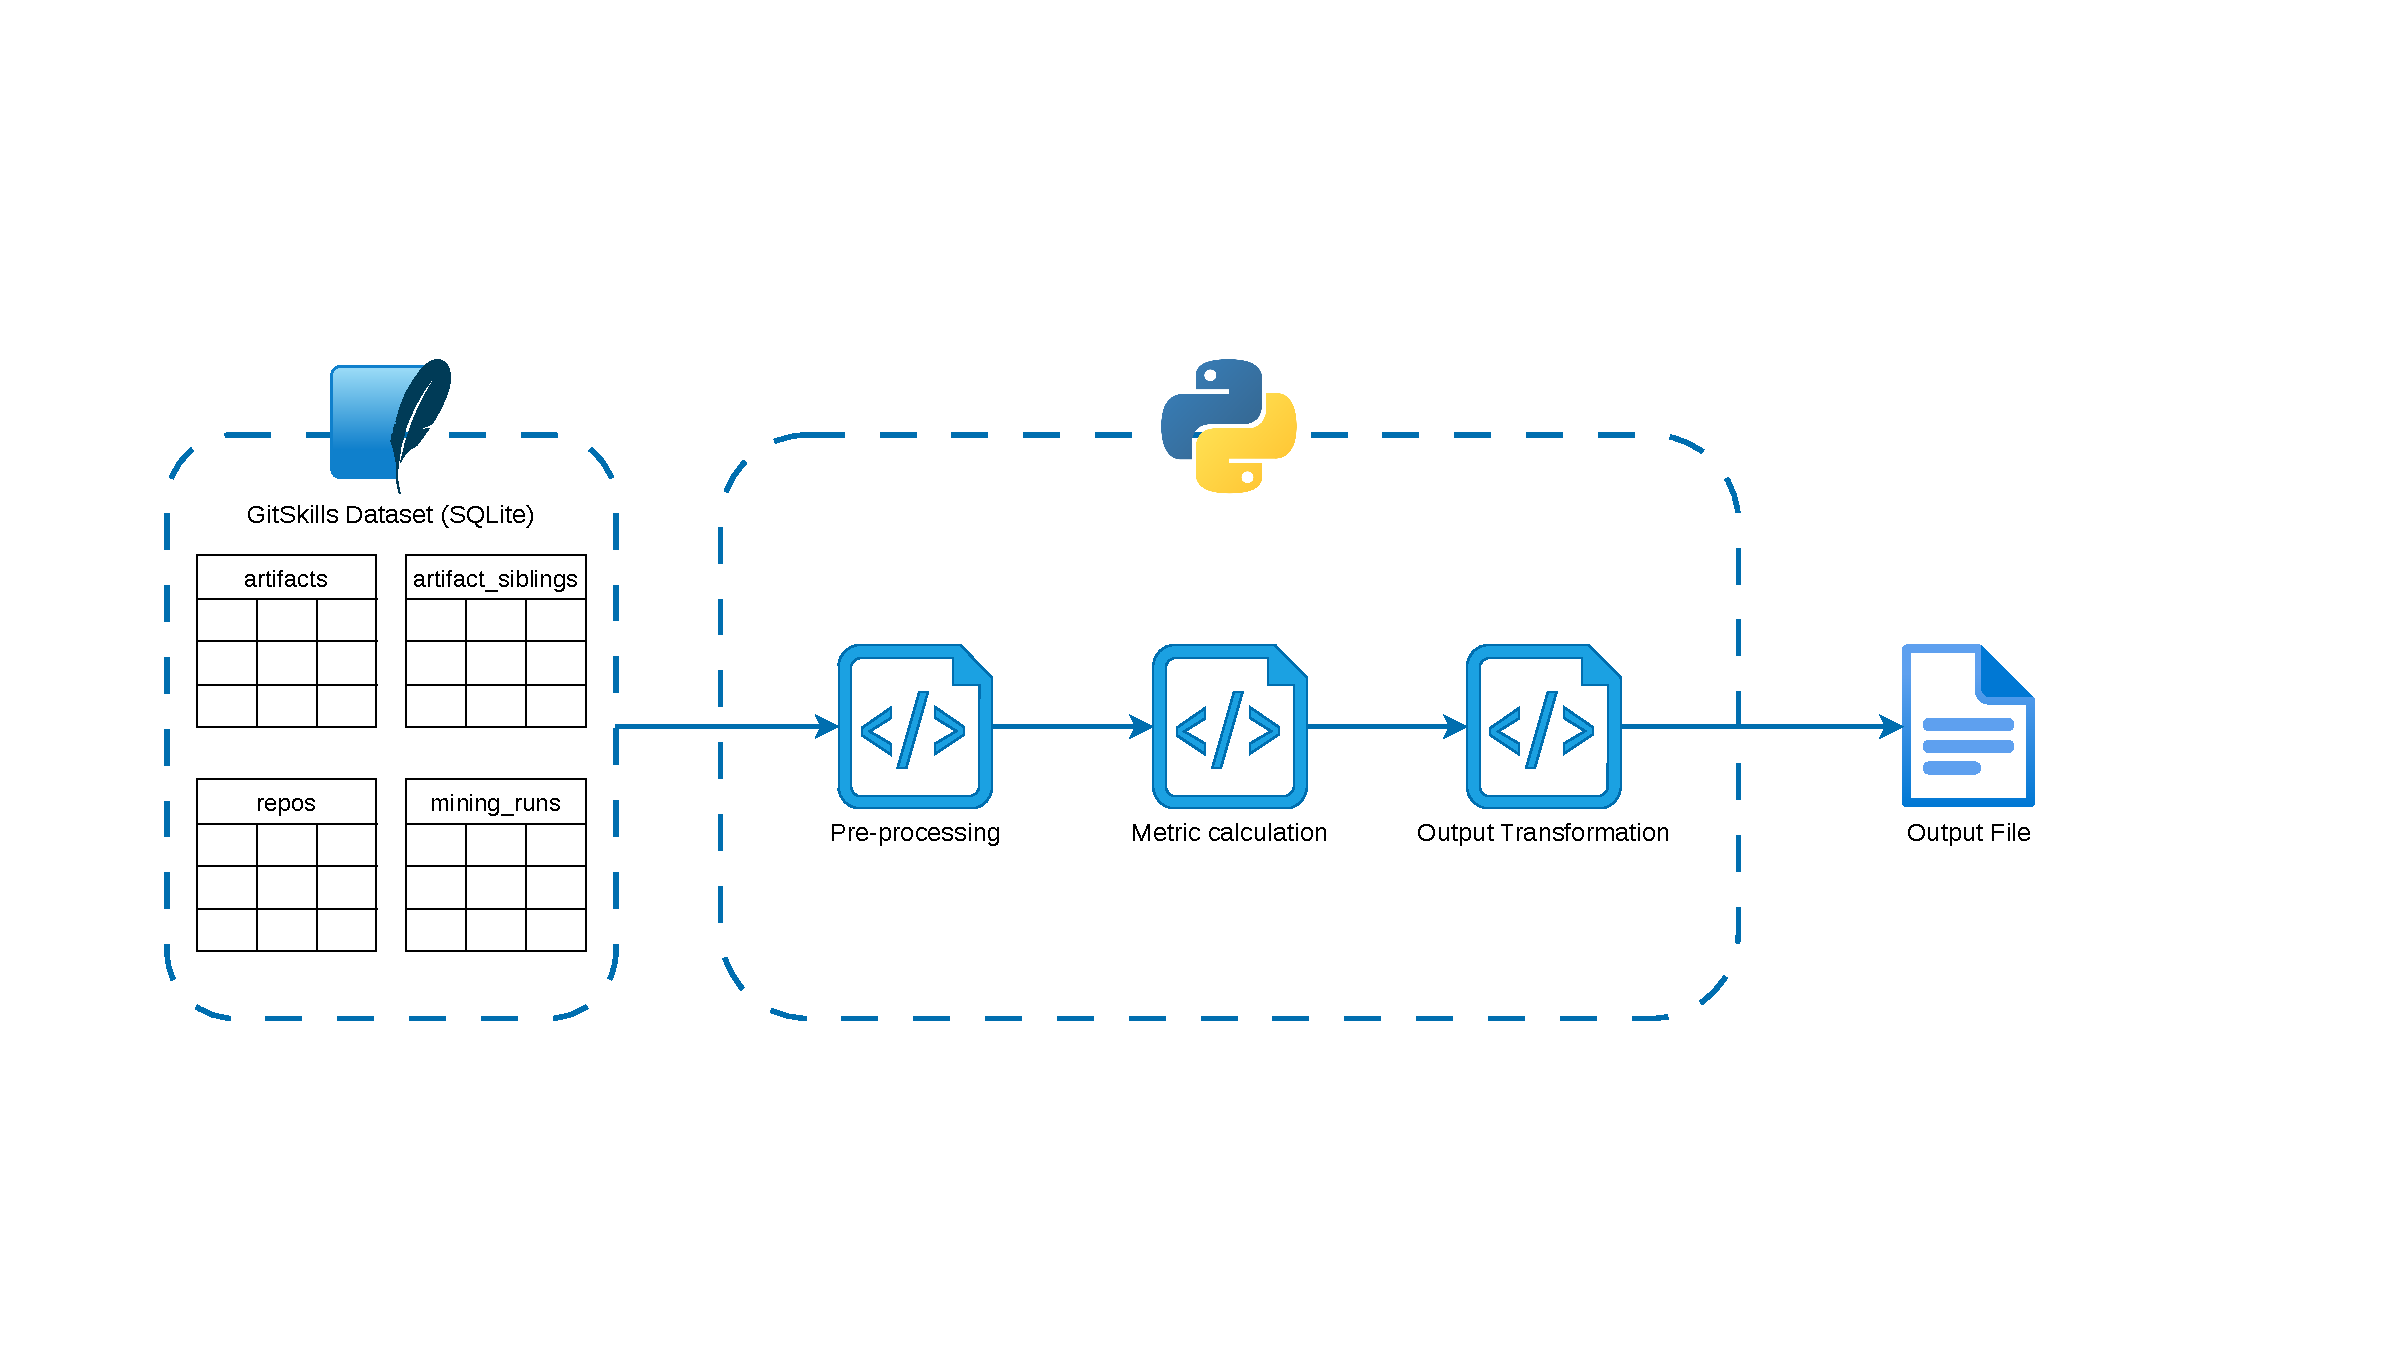
\includegraphics[width=\linewidth]{figures/490CapstoneProposalGeneralFigure1}
\caption{Data flow from the GitSkills tables through the Python pipeline to the final metrics file.}
\label{fig:system}
\end{figure}

\CourseSubsection{Interface and performance specifications}

\begin{singlespace}
\setlength{\LTcapwidth}{\linewidth}
\begin{longtable}{@{}L{0.10\linewidth} L{\dimexpr0.4700000\linewidth-6.0000000\tabcolsep\relax} L{0.22\linewidth} L{0.21\linewidth}@{}}
\caption{Preliminary system specifications.}\label{tab:proposal-specs}\\
\rowcolor{MidGray}
\TableHeader{ID} & \TableHeader{Requirement} & \TableHeader{Target} & \TableHeader{Tolerance} \\
\midrule
\endfirsthead
\rowcolor{MidGray}
\TableHeader{ID} & \TableHeader{Requirement} & \TableHeader{Target} & \TableHeader{Tolerance} \\
\midrule
\endhead
\bottomrule
\endfoot
IF-01 & All four GitSkills tables load into Python with their documented columns & 4 of 4 tables & 0 missing columns \\
\addlinespace[3pt]
IF-02 & Scripts pass data keyed by \texttt{file\_sha}, with no rows lost between stages & 100\% of rows kept & 0 rows \\
\addlinespace[3pt]
IF-03 & Output file holds one row per distinct skill, in Parquet and CSV & 1 row per skill & 0 duplicates \\
\addlinespace[3pt]
PF-01 & Full-dataset run time on one workstation & $\leq$ 24 h & +12 h \\
\addlinespace[3pt]
PF-02 & Peak memory use, kept low through batching & $\leq$ 16 GB & +4 GB \\
\addlinespace[3pt]
PF-03 & Re-running the pipeline reproduces the same metrics & Identical output & 0 differences \\
\addlinespace[3pt]
PF-04 & Precision of cross-copy lineage links on the hand-labelled sample & $\geq$ 0.90 & $-$0.05 \\
\addlinespace[3pt]
PF-05 & Spearman correlation between Flesch--Kincaid grade and the mean human rating on the 100-skill readability sample & $|\rho| \geq$ 0.5 & $-$0.1 \\
\addlinespace[3pt]
PF-06 & Agreement between the two readability raters (Krippendorff's $\alpha$~\cite{krippendorff2004}) & $\geq$ 0.80 & $-$0.13 \\
\end{longtable}
\end{singlespace}

\CourseSubsection{Risks and safety hazards}
The project is purely computational, so it carries no physical, health, or safety hazards.
The main technical risk is the dataset's size (about 44 GB), which is managed by reading the per-table Parquet files in batches rather than loading everything into memory.
Since the data comes from public GitHub repositories with commit authors already anonymized, we will not attempt to identify individuals, and we will respect each repository's license when quoting skill content.
\clearpage

\CourseSection{Design and Production Approach}\label{sec:design}

\CourseSubsection{Metric Development and Analysis}

The following outlines the proposed methods for measuring size, churn, age, clone coverage, and readability, including the data requirements, calculation procedures, and validation approach for each metric.

\noindent\textbf{Size.} \TemplateField{Method and validation approach.}\par
\noindent\textbf{Churn.} \TemplateField{Method and validation approach.}\par
\noindent\textbf{Age.} \TemplateField{Method and validation approach.}\par
\noindent\textbf{Clone Coverage.} \TemplateField{Method and validation approach.}\par
\noindent\textbf{Readability.} \TemplateField{Method and validation approach.}\par

\CourseSubsection{Milestones and Division of Labor}

Progress will be reviewed intermittently during Friday team meetings. Each member will be required to lead at least one milestone, coordinating the work and overseeing its timely completion. Responsibility for implementation and delivery will be shared across the team.

\begin{singlespace}
\setlength{\LTcapwidth}{\linewidth}
\begin{longtable}{@{}L{0.09\linewidth} L{\dimexpr0.55\linewidth-6\tabcolsep\relax} L{0.18\linewidth} L{0.18\linewidth}@{}}
\caption{Proposed technical milestones and ownership.}\label{tab:proposal-milestones}\\
\rowcolor{MidGray}
\TableHeader{ID} & \TableHeader{Milestone} & \TableHeader{Due date} & \TableHeader{Lead}\\
\midrule
\endfirsthead
\endhead
\bottomrule
\endfoot

M1 & Dataset prepared and sample records checked.
& Oct.\ 23, 2026 & Naman\\
\addlinespace[3pt]

M2 & Initial metric calculations checked against reference examples.
& Nov.\ 13, 2026 & James\\
\addlinespace[3pt]

M3 & Supported metrics calculated; initial tables and plots generated.
& Dec.\ 4, 2026 & Faiz\\
\addlinespace[3pt]

M4 & Results reviewed; focused research questions documented.
& Jan.\ 29, 2027 & Noah\\
\addlinespace[3pt]

M5 & Follow-up investigations evaluated; feasible extensions tested.
& Feb.\ 26, 2027 & Naman\\
\addlinespace[3pt]

M6 & Final pipeline validated and results reproduced.
& Mar.\ 12, 2027 & James\\

\end{longtable}
\end{singlespace}

\CourseSubsection{Further Exploration and Contingencies}

Initial findings will guide M5, which may examine instruction structure, bundled scripts and references, or reuse patterns. Additional analyses will depend on relevance, data availability, and remaining time.

Missing data or unreliable metrics will prompt revised methods or a narrower scope. Processing limits will be managed through batching or documented sampling to control time and costs. If delays threaten validation, tasks will be reassigned and optional investigations deferred. Resulting limitations will be documented.

\clearpage
\CourseSection{Testing and Evaluation}\label{sec:testing}

\Guidance{Describe how the team expects to test the proposed system. The purpose
of this section is to show that testing has been considered, not to provide a
complete test procedure. (This you will do in the blueprint.) Use a diagram to communicate the overall test approach
and briefly explain the expected evidence of success.}

\begin{figure}[htbp]
\centering
\FigurePlaceholder{Insert diagrms showing the test environments, and link IDs to the requirements and specifications.\\
Show what will be tested, the main inputs and measurements,
and how the results connect to the project requirements.}
\caption{\TemplateField{Proposed system testing approach...be more specific here.}}
\label{fig:test-approach}
\end{figure}

\begin{singlespace}
\begin{tabularx}{\linewidth}{@{}L{0.18\linewidth}YY@{}}
\rowcolor{MidGray}
\TableHeader{Requirement} &
\TableHeader{Proposed test} &
\TableHeader{Expected evidence of success} \\
\midrule

\TemplateField{ID} &
\TemplateField{Briefly describe the planned test.} &
\TemplateField{State the expected result or pass criterion.} \\

\bottomrule
\end{tabularx}
\end{singlespace}

\Guidance{List as many verification and validation tests as you can think of at this time. Briefly identify any equipment, software, facilities, or special
conditions expected to be needed. Explain how the tests will help
determine whether the final system meets its main requirements (verification) and stakeholder
needs (validation).}

\clearpage
\CourseSection{Resource Requirements}\label{sec:resources}
\CourseSubsection{Scheduling access to resources}
\Guidance{Connect the technical milestones to laboratory space, equipment, fabrication, software, subscriptions, repositories, and other resources. Discuss access with the supervisor and include booking or lead-time requirements.}

\begin{singlespace}
\setlength{\LTcapwidth}{\linewidth}
\begin{longtable}{@{}L{0.14\linewidth} L{\dimexpr0.6100000\linewidth-4.0000000\tabcolsep\relax} L{0.25\linewidth}@{}}
\caption{Resource access by milestone.}\label{tab:resource-access}\\
\rowcolor{MidGray}
\TableHeader{Milestone} & \TableHeader{Resource / source} & \TableHeader{Access date / lead time} \\
\midrule
\endfirsthead
\rowcolor{MidGray}
\TableHeader{Milestone} & \TableHeader{Resource / source} & \TableHeader{Access date / lead time} \\
\midrule
\endhead
\bottomrule
\endfoot
% Add or replace data rows below. Keep the matching column separators.
M1 & \TemplateField{Tools and design resources} & \TemplateField{Date; lead time} \\
\addlinespace[3pt]
M2--M3 & \TemplateField{Lab; equipment; fabrication} & \TemplateField{Date; booking} \\
\addlinespace[3pt]
M4 & \TemplateField{Test equipment and facilities} & \TemplateField{Date; booking} \\
\end{longtable}
\end{singlespace}

\Guidance{You can also relate each resource to the verification tests, or any other aspect of your report. Try to make use of labels / IDs so that they can be referenced consistently across the report.}

\CourseSubsection{Materials and other resources}
\Guidance{Estimate costs in \BudgetCurrency. Include quantities and the basis for estimates; identify resources supplied through existing access. Include tax, shipping, and contingency where applicable.}

\begin{singlespace}
\setlength{\LTcapwidth}{\linewidth}
\begin{longtable}{@{}L{\dimexpr0.5300000\linewidth-6.0000000\tabcolsep\relax} C{0.09\linewidth} L{0.18\linewidth} L{0.20\linewidth}@{}}
\caption{Preliminary cost estimate (\BudgetCurrency).}\label{tab:proposal-budget}\\
\rowcolor{MidGray}
\TableHeader{Item / source} & \TableHeader{Qty.} & \TableHeader{Unit cost} & \TableHeader{Total} \\
\midrule
\endfirsthead
\rowcolor{MidGray}
\TableHeader{Item / source} & \TableHeader{Qty.} & \TableHeader{Unit cost} & \TableHeader{Total} \\
\midrule
\endhead
\bottomrule
\endfoot
% Add or replace data rows below. Keep the matching column separators.
\TemplateField{Hardware / supplier} & \TemplateField{n} & \TemplateField{Cost} & \TemplateField{Cost} \\
\addlinespace[3pt]
\TemplateField{Software / service / access} & \TemplateField{n} & \TemplateField{Cost} & \TemplateField{Cost} \\
\addlinespace[3pt]
\TemplateField{Tax; shipping; contingency} &  &  & \TemplateField{Cost} \\
\addlinespace[3pt]
\textbf{Estimated total} &  &  & \TemplateField{Total} \\
\end{longtable}
\end{singlespace}


\TemplateField{State the cost assumptions, access arrangements, and supervisor or industry contributions. Explain the funding and availability needed to complete the project.}
\clearpage

\CourseSection{Conclusion}\label{sec:conclusion}
\Guidance{Summarize the project and the evidence established in Sections 1--5. End with the expected contribution and the team's readiness to proceed.}

This project aims to examine size, churn, age, clone coverage, and readability within AI agent skills using the GitSkills dataset. The team plans to study how these skills are developed and maintained, and whether traditional software engineering metrics can be meaningfully applied to them. The final system will be a Python analysis pipeline that processes the dataset and calculates metrics based on the available fields.

Development will follow six milestones (M1–M6). M1 focuses on dataset preparation and verification of sample records. Next, M2 involves the initial metric calculations and checking them against reference examples. Once the methods have been established, the team will calculate the supported metrics across the dataset and generate preliminary tables and visualizations (M3). This is followed by M4, which involves reviewing results and documenting focused research questions. Based on these findings, the team will investigate follow-up questions and potential extensions during M5. Finally, the pipeline will undergo validation and reproducibility testing in M6. The pipeline will be designed to process the full dataset within 24 hours while using no more than 16 GB of memory. Testing will include unit tests, integration tests, and reproducibility checks to ensure the calculated metrics are accurate and consistent. Since the project relies on publicly available data and open-source tools, the estimated total cost is \$0 CAD.

The expected outcome of the project is to identify and document meaningful metrics that can help developers and researchers better understand AI agent skills and how they evolve. The full scope of the project will depend on the results of preliminary analysis, as focused research questions will be established during M4 and investigated further during M5. Although this makes part of the project's scope open-ended, the team has established a clear development plan, assigned milestones, and identified the resources needed for success. With initial pilot analyses already completed, the team is prepared to move forward with implementation and validation.

\CourseSection{References}\label{sec:references}

\Guidance{Replace these entries with the sources used in the proposal. Include previous project reports, papers, books, data sheets, and web resources as appropriate. Supply enough information to retrieve each source. Cite external claims, data, and adapted figures, and record permission or license details for reused material.}

\printbibliography[heading=none]

\clearpage
\ifincludeappendices
  \appendix
  \CourseSection{Supporting Schedule and Technical Material}\label{app:schedule}
\Guidance{Use appendices for a detailed timeline or Gantt chart, supporting calculations, data sheets, or additional diagrams. Cite each included appendix from the body.}

\TemplateField{Insert the detailed schedule or supporting material.}

% A second appendix can be a separate file, added after this one in main.tex:
% \input{sections/12-appendix-calculations}
% Start that file with \CourseSection{Supporting Calculations}.

  \clearpage
\CourseSection{Readability Pilot}\label{app:readability-pilot}

We ran the readability method on the official 13,000-skill GitSkills sample to check that it is feasible and to choose the preprocessing.
Of the 13,000 distinct skills, 237 were not named exactly \texttt{SKILL.md}, 1,566 had invalid front matter, 555 were too short (a body under 300 characters or fewer than 30 words of prose), and 2,328 were not in English.
This left 8,314 skills from 5,567 repositories.
Figure~\ref{fig:readability-pilot}a shows why the Markdown must be converted into sentences before scoring: on raw text, each bullet list counts as one long sentence, and the median grade rises from 8.6 to 12.2.
Figure~\ref{fig:readability-pilot}b shows that skill sentences are short (a median of 9 words), but formulas that weight word length, such as Coleman--Liau, place the same text near grade 13, which reflects technical vocabulary.
Descriptions are usually a single long sentence, and they read about four grades harder than the bodies.
The pilot code uses textstat~\cite{textstat}; whole-sample scoring took about 6\,ms per skill on one laptop core, or roughly 3\,h for the full 1.88 million distinct skills.

\begin{figure}[htbp]
\centering
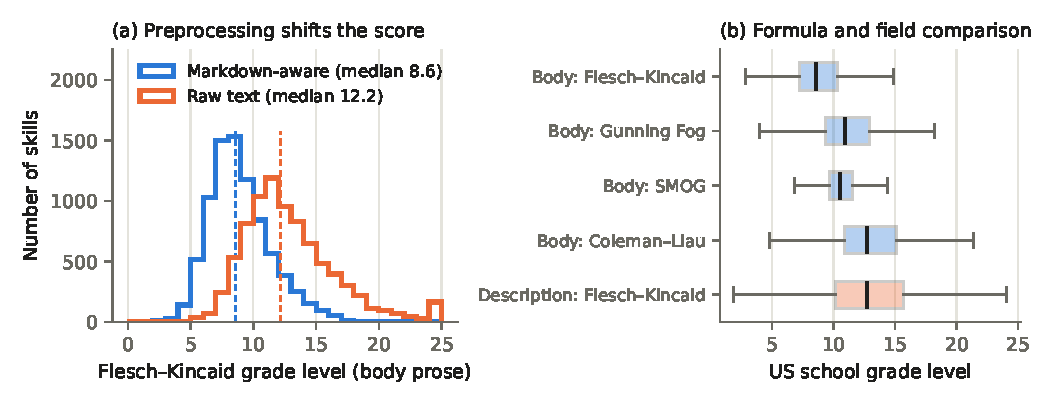
\includegraphics[width=\linewidth,keepaspectratio]{figures/readability-pilot.pdf}
\caption{Readability pilot on 8,314 English skills from the 13,000-skill GitSkills sample. (a)~Flesch--Kincaid grade of the body prose, with the Markdown converted to sentences and as raw text. (b)~Body grade under four formulas, and Flesch--Kincaid grade of the front-matter description. Boxes show the interquartile range, and whiskers extend to 1.5 times the IQR.}
\label{fig:readability-pilot}
\end{figure}

  % % Engineering diagram selection guide for an EE/CompE capstone report.
% Include this file with: \input{engineering-diagram-guide}
% This section uses the template's \CourseSection, \CourseSubsection,
% \Guidance, \TableHeader, \FigurePlaceholder, and L column macros.
% It also assumes longtable, booktabs, xcolor, and setspace are loaded.

\CourseSection{Engineering Diagram Selection Guide}\label{sec:diagram-guide}

\Guidance{Use this section as a catalog for selecting engineering diagrams. Retain the diagram types that communicate the project requirements, architecture, behavior, implementation, analysis, verification, safety, and execution plan. Introduce every retained diagram in the report text and explain the engineering decisions represented by its elements and relationships. Use consistent subsystem names, interface names, requirement IDs, units, signal directions, and terminology across the complete report.}

\CourseSubsection{Diagram selection principles}

\Guidance{Each diagram should answer a defined engineering question. A context diagram answers what interacts with the system; a functional architecture answers what the system must do; a physical architecture answers where each function is implemented; a state or sequence diagram answers how behavior changes; a schematic answers how electrical components connect; and a test diagram answers how performance will be measured. Combine diagrams when the shared view remains legible and separate diagrams when each view serves a distinct audience or design question.}

For each retained diagram, provide the following information where applicable:
\begin{itemize}
    \item a descriptive title and a unique \verb|\label|;
    \item a clearly defined system boundary, scope, or level of abstraction;
    \item labeled components, functions, states, nodes, or actors;
    \item directed and labeled connections, transitions, messages, or flows;
    \item signal type, protocol, voltage, current, power, frequency, sample rate, bit width, data rate, impedance, timing, or physical units;
    \item operating assumptions, constraints, tolerances, and exceptional conditions;
    \item requirement IDs, interface IDs, test IDs, or component reference designators when traceability is useful;
    \item a caption that states the relationship or engineering conclusion represented by the figure.
\end{itemize}

\CourseSubsection{System definition and architecture diagrams}

\begin{singlespace}
\setlength{\LTcapwidth}{\linewidth}
\begin{longtable}{@{}L{0.17\linewidth} L{0.23\linewidth} L{0.32\linewidth} L{\dimexpr0.28\linewidth-6\tabcolsep\relax}@{}}
\caption{System definition and architecture diagrams.}\label{tab:system-architecture-diagrams}\\
\rowcolor{MidGray}
\TableHeader{Diagram} & \TableHeader{Purpose} & \TableHeader{Required content} & \TableHeader{EE or CompE example} \\
\midrule
\endfirsthead
\rowcolor{MidGray}
\TableHeader{Diagram} & \TableHeader{Purpose} & \TableHeader{Required content} & \TableHeader{EE or CompE example} \\
\midrule
\endhead
\bottomrule
\endfoot
System context & Defines the system boundary and external environment. & System under design, users, external devices, power sources, physical processes, networks, and labeled incoming and outgoing flows. & A motor controller connected to a battery, motor, encoder, operator, emergency stop, and service computer. \\
\addlinespace[3pt]
Use-case & Identifies capabilities delivered to users or external systems. & Actors, use cases, system boundary, associations, and included or extended behavior where those relationships clarify scope. & A technician configures sampling, an operator starts acquisition, and a cloud service receives telemetry. \\
\addlinespace[3pt]
Stakeholder map & Relates stakeholders to needs, decisions, and system effects. & Stakeholder groups, interests, authority, affected requirements, and communication paths. & Operators prioritize usability, technicians prioritize service access, and safety personnel approve protective functions. \\
\addlinespace[3pt]
Functional decomposition & Breaks a top-level mission into implementable functions. & Parent function, subordinate functions, hierarchy, inputs, outputs, and allocation identifiers when available. & Measure optical power decomposed into detection, amplification, filtering, conversion, calibration, storage, and display. \\
\addlinespace[3pt]
System block diagram & Summarizes the major subsystems and their relationships. & Subsystem blocks, labeled interfaces, flow direction, signal or energy type, and system boundary. & Sensor board, FPGA board, processor, power board, communications module, and host application. \\
\addlinespace[3pt]
Functional-flow block diagram & Shows the logical order, concurrency, and branching of functions. & Functions, sequence numbers, branches, parallel paths, entry and exit conditions, and feedback loops. & Initialize hardware, calibrate channels, acquire samples, process data, transmit results, and monitor faults. \\
\addlinespace[3pt]
Internal block or interface diagram & Defines connections among internal parts. & Parts, ports, connectors, interface names, directions, item flows, protocols, and electrical constraints. & MCU and FPGA connected by SPI, DMA request, reset, interrupt, clock, and shared power rails. \\
\addlinespace[3pt]
Logical architecture & Groups functions into technology-independent logical elements. & Logical components, responsibilities, provided and required services, data stores, and logical interfaces. & Acquisition service, control service, safety monitor, data logger, and communications service. \\
\addlinespace[3pt]
Physical architecture & Maps system responsibilities onto physical components. & Boards, processors, sensors, actuators, memories, connectors, enclosures, and allocation of functions to hardware. & Filtering assigned to an FPGA, supervisory control assigned to an MCU, and visualization assigned to a host PC. \\
\addlinespace[3pt]
Allocation diagram & Traces functions, requirements, or software onto implementation elements. & Source elements, target elements, allocation relationships, IDs, and unresolved allocations. & Requirement R-14 allocated to an ADC, anti-alias filter, FPGA decimator, and verification test T-14. \\
\addlinespace[3pt]
Interface control diagram & Provides a controlled definition of a subsystem boundary. & Interface ID, source, destination, connector or medium, pins, signals, voltage levels, protocol, units, timing, and ownership. & A 40-pin board connector carrying LVDS data, clocks, I\textsuperscript{2}C control, reset, and power. \\
\addlinespace[3pt]
Requirements traceability diagram & Connects stakeholder needs, requirements, design elements, and tests. & Requirement IDs, derivation, satisfaction relationships, verification methods, and test IDs. & A latency requirement satisfied by FPGA processing and verified by oscilloscope measurement. \\
\addlinespace[3pt]
System-of-systems diagram & Shows independently operated systems cooperating toward a broader capability. & Constituent systems, ownership, exchanged services, network boundaries, and operational dependencies. & Distributed sensor nodes, an edge gateway, a campus network, and a cloud analytics platform. \\
\end{longtable}
\end{singlespace}

\CourseSubsection{Electrical and electronic design diagrams}

\begin{singlespace}
\setlength{\LTcapwidth}{\linewidth}
\begin{longtable}{@{}L{0.17\linewidth} L{0.23\linewidth} L{0.32\linewidth} L{\dimexpr0.28\linewidth-6\tabcolsep\relax}@{}}
\caption{Electrical and electronic design diagrams.}\label{tab:electrical-diagrams}\\
\rowcolor{MidGray}
\TableHeader{Diagram} & \TableHeader{Purpose} & \TableHeader{Required content} & \TableHeader{EE or CompE example} \\
\midrule
\endfirsthead
\rowcolor{MidGray}
\TableHeader{Diagram} & \TableHeader{Purpose} & \TableHeader{Required content} & \TableHeader{EE or CompE example} \\
\midrule
\endhead
\bottomrule
\endfoot
Circuit schematic & Defines exact electrical connectivity and component relationships. & Reference designators, values, part numbers where relevant, nets, rails, grounds, connector pins, test points, and sheet references. & Photodiode transimpedance amplifier with bias, compensation, protection, and ADC driver. \\
\addlinespace[3pt]
Single-line diagram & Summarizes a multiphase or high-power electrical system with one line per circuit path. & Sources, buses, breakers, transformers, converters, loads, ratings, protection, and grounding. & Three-phase source feeding a rectifier, DC link, inverter, motor, and protective devices. \\
\addlinespace[3pt]
Power-tree diagram & Shows generation and distribution of supply rails. & Sources, protection, converters, regulators, switches, rails, loads, voltage ranges, current estimates, efficiency, and sequencing. & USB-C input converted to 12~V, 5~V, 3.3~V, 1.8~V, and FPGA core rails. \\
\addlinespace[3pt]
Energy-flow diagram & Shows conversion, storage, delivery, and recovery of energy. & Energy sources, conversion stages, storage elements, loads, losses, efficiencies, and bidirectional paths. & Battery, DC--DC converter, inverter, motor, mechanical load, and regenerative braking path. \\
\addlinespace[3pt]
Signal-chain diagram & Shows signal conditioning and conversion from source to destination. & Sensor or source, protection, gain, filtering, ADC or DAC, digital processing, sample rates, bandwidths, ranges, and noise-sensitive boundaries. & Photodiode, transimpedance amplifier, low-pass filter, ADC, FPGA filter, and Ethernet output. \\
\addlinespace[3pt]
Analog signal-flow diagram & Describes gain, filtering, feedback, and loading across an analog path. & Stages, gains, transfer functions, impedances, noise contributions, bandwidth, and signal ranges. & Microphone preamplifier followed by high-pass filtering, programmable gain, and audio ADC. \\
\addlinespace[3pt]
Grounding and isolation diagram & Defines reference domains, shielding, and safety or noise barriers. & Protective earth, chassis, analog and digital references, isolated domains, shields, return paths, and isolation ratings. & Isolated CAN interface between a high-voltage inverter controller and a low-voltage service tool. \\
\addlinespace[3pt]
Return-current path diagram & Shows the physical return path associated with a high-frequency or high-current signal. & Forward path, reference plane, discontinuities, stitching vias, connector returns, and current-loop area. & FPGA clock crossing a split plane and returning through a nearby stitching capacitor. \\
\addlinespace[3pt]
Timing diagram & Defines logic-level relationships and timing constraints. & Clock, reset, enable, chip select, address, data, interrupt, active levels, setup time, hold time, pulse width, and latency. & SPI transaction that starts an ADC conversion and reads a 24-bit result. \\
\addlinespace[3pt]
Waveform diagram & Communicates expected or measured voltage, current, or optical behavior over time. & Axes, units, trigger or reference event, operating condition, limits, annotations, and measurement location. & Gate voltage, switch-node voltage, and inductor current during a converter switching cycle. \\
\addlinespace[3pt]
PCB stack-up & Defines board layers and controlled electromagnetic geometry. & Copper layers, dielectric materials, thicknesses, reference planes, impedance targets, via structures, and total thickness. & Eight-layer mixed-signal board with dedicated analog and digital reference planes. \\
\addlinespace[3pt]
PCB floorplan or placement diagram & Communicates functional partitioning and component placement. & Board outline, connectors, major devices, power stages, analog, digital and RF regions, thermal zones, and keep-outs. & ADC placed beside its driver, FPGA beside DDR memory, and switching regulators separated from the analog front end. \\
\addlinespace[3pt]
Critical-routing diagram & Identifies nets requiring controlled geometry or matched routing. & Differential pairs, impedance, length or skew limits, termination, layer changes, return vias, and spacing constraints. & DDR byte lanes, PCIe pairs, LVDS ADC lanes, and reference clocks. \\
\addlinespace[3pt]
Wiring or harness diagram & Defines cable construction and point-to-point connectivity. & Connector IDs, pin mappings, wire gauges, colors, lengths, twists, shields, splices, labels, and routing constraints. & Enclosure harness connecting the controller, encoder, motor driver, fan, and emergency stop. \\
\addlinespace[3pt]
Connector pinout & Provides a compact definition of connector signals. & Pin numbers, names, direction, voltage, current limit, logic standard, mating connector, and reserved pins. & Debug connector carrying JTAG, UART, reset, 3.3~V, and ground. \\
\addlinespace[3pt]
RF or optical link budget & Accounts for gains, losses, noise, and operating margin. & Transmit power, coupling loss, path loss, gain, receiver sensitivity, noise figure, bandwidth, and margin. & Optical transmitter, fiber and connector losses, photoreceiver sensitivity, and required power margin. \\
\addlinespace[3pt]
Thermal-flow diagram & Shows heat generation and transfer to the environment. & Heat sources, dissipation, thermal resistance, junction and ambient limits, heat spreaders, heat sinks, airflow, and enclosure paths. & FPGA and regulators conducting heat through thermal vias to a heat spreader and forced-air path. \\
\addlinespace[3pt]
EMI or EMC coupling diagram & Identifies emission sources, coupling paths, and susceptible circuits. & Noise source, conductive and radiated paths, antennas, common-mode paths, filters, shields, and affected nodes. & Switching converter noise coupling through a cable shield into a low-level analog measurement channel. \\
\end{longtable}
\end{singlespace}

\CourseSubsection{Firmware, FPGA, and software diagrams}

\begin{singlespace}
\setlength{\LTcapwidth}{\linewidth}
\begin{longtable}{@{}L{0.17\linewidth} L{0.23\linewidth} L{0.32\linewidth} L{\dimexpr0.28\linewidth-6\tabcolsep\relax}@{}}
\caption{Firmware, FPGA, and software diagrams.}\label{tab:computing-diagrams}\\
\rowcolor{MidGray}
\TableHeader{Diagram} & \TableHeader{Purpose} & \TableHeader{Required content} & \TableHeader{EE or CompE example} \\
\midrule
\endfirsthead
\rowcolor{MidGray}
\TableHeader{Diagram} & \TableHeader{Purpose} & \TableHeader{Required content} & \TableHeader{EE or CompE example} \\
\midrule
\endhead
\bottomrule
\endfoot
Flowchart & Shows algorithmic sequence, decisions, and iteration. & Start and end points, operations, decisions, loops, inputs, outputs, and error paths. & Read sensors, validate ranges, calculate control output, update actuator, and log faults. \\
\addlinespace[3pt]
Activity diagram & Shows workflows with branching, concurrency, and responsibility partitions. & Actions, decisions, forks, joins, object flows, start and completion nodes, and swimlanes where ownership matters. & Firmware and host software concurrently acquire, process, display, and archive measurements. \\
\addlinespace[3pt]
State-machine diagram & Defines mode-dependent behavior. & Initial state, states, events, guards, actions, timeouts, fault states, safe states, and recovery transitions. & Reset, initialization, idle, acquisition, processing, communication, fault, and recovery. \\
\addlinespace[3pt]
Sequence diagram & Shows time-ordered messages among components. & Participants, messages, return values, asynchronous events, loops, alternatives, timeouts, retries, and concurrency. & MCU configures an ADC, arms DMA, receives an interrupt, and transfers a data block to a host. \\
\addlinespace[3pt]
Data-flow diagram & Shows creation, transformation, storage, and delivery of data. & External entities, processes, data stores, named data flows, and level of decomposition. & Camera frames pass through correction, feature extraction, buffering, compression, and network transmission. \\
\addlinespace[3pt]
Software component diagram & Defines software modules and dependencies. & Components, provided and required interfaces, APIs, libraries, services, drivers, and dependency direction. & Sensor driver, estimator, controller, logger, communications stack, and user-interface service. \\
\addlinespace[3pt]
Deployment diagram & Maps software artifacts onto execution nodes. & Processors, operating environments, firmware images, services, applications, storage, and communication links. & FPGA bitstream, MCU firmware, Linux service, desktop application, and cloud database. \\
\addlinespace[3pt]
Class diagram & Describes object-oriented software structure. & Classes, attributes, operations, inheritance, associations, composition, and multiplicity. & Device, Sensor, Channel, Calibration, Measurement, and Transport classes. \\
\addlinespace[3pt]
Entity--relationship diagram & Defines persistent data structure and relationships. & Entities, attributes, keys, relationships, cardinality, and constraints. & Devices, calibration records, test runs, channels, measurements, and users. \\
\addlinespace[3pt]
FPGA datapath diagram & Shows registered data transformations and pipeline structure. & Registers, arithmetic units, multiplexers, memories, pipeline stages, bus widths, valid-ready signals, and clock domains. & ADC samples pass through scaling, FIR filtering, decimation, FFT, detection, and packet framing. \\
\addlinespace[3pt]
FPGA control-path diagram & Shows logic that configures and sequences the datapath. & State machines, counters, enables, selectors, status flags, handshakes, reset behavior, and error handling. & Controller schedules buffer fills, FFT starts, result transfers, and overflow recovery. \\
\addlinespace[3pt]
Clock and reset architecture & Defines clock generation, distribution, domain crossings, and reset release. & Oscillators, PLLs, frequencies, clock domains, gating, CDC mechanisms, reset sources, synchronizers, and sequencing. & 100-MHz control domain, 250-MHz signal-processing domain, asynchronous ADC clock, and synchronized resets. \\
\addlinespace[3pt]
Memory map & Allocates processor or FPGA address space. & Address ranges, memory and peripheral regions, aliases, permissions, reserved areas, and bus ownership. & Flash, SRAM, DMA buffers, UART, timers, ADC control, and FPGA register window. \\
\addlinespace[3pt]
Register map & Defines individual control and status registers. & Offset, name, width, access type, reset value, bit fields, side effects, and description. & FPGA control register with enable, reset, interrupt mask, overflow, and operating-mode fields. \\
\addlinespace[3pt]
Interrupt architecture & Shows interrupt sources, priorities, and service relationships. & Sources, vectors, priorities, masking, preemption, handlers, latency targets, and shared-resource effects. & Emergency stop has priority over ADC completion, DMA completion, timer, UART, and background events. \\
\addlinespace[3pt]
Task-scheduling diagram & Shows concurrent or periodic software execution. & Tasks, periods, deadlines, priorities, execution times, dependencies, queues, mutexes, and processor utilization. & Control at 1~kHz, acquisition at 20~kHz, telemetry at 10~Hz, and diagnostics at 1~Hz. \\
\addlinespace[3pt]
Call graph & Shows function or procedure invocation relationships. & Functions, callers, callees, recursion where applicable, library boundaries, and critical call paths. & Interrupt handler invokes buffer management, filtering, fault checks, and event notification. \\
\addlinespace[3pt]
Cybersecurity trust-boundary diagram & Shows protected assets and crossings between trust zones. & Assets, users, devices, trust boundaries, authentication points, encrypted links, attack surfaces, and privileged flows. & Sensor node, maintenance port, gateway, local network, cloud API, credential store, and update service. \\
\end{longtable}
\end{singlespace}

\CourseSubsection{Control, signal-processing, and communications diagrams}

\begin{singlespace}
\setlength{\LTcapwidth}{\linewidth}
\begin{longtable}{@{}L{0.17\linewidth} L{0.23\linewidth} L{0.32\linewidth} L{\dimexpr0.28\linewidth-6\tabcolsep\relax}@{}}
\caption{Control, signal-processing, and communications diagrams.}\label{tab:analysis-diagrams}\\
\rowcolor{MidGray}
\TableHeader{Diagram} & \TableHeader{Purpose} & \TableHeader{Required content} & \TableHeader{EE or CompE example} \\
\midrule
\endfirsthead
\rowcolor{MidGray}
\TableHeader{Diagram} & \TableHeader{Purpose} & \TableHeader{Required content} & \TableHeader{EE or CompE example} \\
\midrule
\endhead
\bottomrule
\endfoot
Control-loop diagram & Defines closed-loop regulation and disturbance paths. & Reference, summing junctions, controller, actuator, plant, sensor, feedback, disturbances, noise, and controlled output. & Current and speed loops for a permanent-magnet motor drive. \\
\addlinespace[3pt]
Signal-flow graph & Represents linear relationships among system variables. & Nodes, directed branches, gains or transfer functions, feedback paths, and input-output variables. & Small-signal model of a converter control loop. \\
\addlinespace[3pt]
Bond graph & Represents energy exchange across multiple physical domains. & Effort and flow variables, sources, storage, dissipation, transformers, gyrators, and junctions. & Electromechanical model of a motor, shaft, gear train, and load. \\
\addlinespace[3pt]
Bode plot & Shows frequency-dependent magnitude and phase. & Frequency axis, magnitude, phase, operating condition, crossover frequencies, bandwidth, gain margin, phase margin, and design limits. & Compensated power-converter loop with required phase margin. \\
\addlinespace[3pt]
Nyquist plot & Assesses closed-loop stability from open-loop frequency response. & Complex-plane locus, direction, critical point, encirclement interpretation, and operating condition. & Robustness analysis of a plant with transport delay. \\
\addlinespace[3pt]
Pole--zero plot & Shows dynamic modes and stability. & Poles, zeros, stability boundary, dominant modes, damping, natural frequency, and parameter condition. & Digital controller and sampled plant poles in the (z)-plane. \\
\addlinespace[3pt]
Root-locus plot & Shows movement of closed-loop poles as gain changes. & Pole and zero locations, locus branches, gain values, damping lines, and selected operating point. & Controller-gain selection for a motor-position loop. \\
\addlinespace[3pt]
Time-response plot & Demonstrates transient or steady-state performance. & Input command or disturbance, output response, axes, units, rise time, overshoot, settling time, error, and limits. & Temperature controller response to a setpoint step and load disturbance. \\
\addlinespace[3pt]
Signal-processing pipeline & Shows ordered transformations applied to sampled data. & Sampling, buffering, windowing, filtering, transforms, feature extraction, estimation, data types, rates, and latency. & ADC samples pass through calibration, FIR filter, FFT, peak detection, and packetization. \\
\addlinespace[3pt]
Spectrum or spectral-density plot & Shows signal or noise content versus frequency. & Frequency axis, amplitude or density units, resolution bandwidth, window, averaging, noise floor, tones, and limits. & Output-noise density of a transimpedance amplifier. \\
\addlinespace[3pt]
Spectrogram & Shows spectral content changing with time. & Time, frequency, magnitude scale, window length, overlap, sample rate, and annotated events. & Motor vibration signature during acceleration and steady operation. \\
\addlinespace[3pt]
Constellation diagram & Shows received digital-modulation symbols in the I/Q plane. & Ideal symbols, measured samples, modulation type, EVM, decision boundaries, and identified impairments. & QPSK telemetry link showing phase error, gain imbalance, and noise. \\
\addlinespace[3pt]
Eye diagram & Shows aggregate timing and amplitude margin of a digital link. & Unit interval, eye height, eye width, crossing levels, jitter, noise, mask, and sampling point. & LVDS or optical receiver eye at the target data rate. \\
\addlinespace[3pt]
Channel model & Represents propagation, loss, interference, and noise. & Transmitter, medium, transfer function, attenuation, delay, multipath, noise, interference, and receiver. & Wireless sensor link through an indoor multipath channel. \\
\addlinespace[3pt]
Protocol-stack diagram & Shows communication responsibilities by layer. & Application, transport, network, link, and physical layers; protocols; interfaces; encapsulation; and security functions. & Sensor messages transported through MQTT, TCP, IP, Wi-Fi, and RF. \\
\end{longtable}
\end{singlespace}

\CourseSubsection{Mechanical integration and user-interface diagrams}

\begin{singlespace}
\setlength{\LTcapwidth}{\linewidth}
\begin{longtable}{@{}L{0.17\linewidth} L{0.23\linewidth} L{0.32\linewidth} L{\dimexpr0.28\linewidth-6\tabcolsep\relax}@{}}
\caption{Mechanical integration and user-interface diagrams.}\label{tab:physical-diagrams}\\
\rowcolor{MidGray}
\TableHeader{Diagram} & \TableHeader{Purpose} & \TableHeader{Required content} & \TableHeader{EE or CompE example} \\
\midrule
\endfirsthead
\rowcolor{MidGray}
\TableHeader{Diagram} & \TableHeader{Purpose} & \TableHeader{Required content} & \TableHeader{EE or CompE example} \\
\midrule
\endhead
\bottomrule
\endfoot
Mechanical assembly & Shows how physical parts fit and are retained. & Enclosure, boards, sensors, connectors, fasteners, mounting points, orientation, dimensions, and assembly references. & Controller PCB mounted above a power board with standoffs and airflow clearance. \\
\addlinespace[3pt]
Exploded view & Communicates part order and assembly sequence. & Separated parts, item numbers, orientation, fasteners, seals, and bill-of-material references. & Instrument enclosure, display window, keypad, PCB, battery, gasket, and rear cover. \\
\addlinespace[3pt]
Dimensioned drawing & Defines manufacturable geometry and tolerances. & Views, dimensions, tolerances, datums, hole patterns, materials, finish, and revision. & Front panel with display opening, connector cutouts, mounting holes, and labels. \\
\addlinespace[3pt]
Cable-routing diagram & Defines cable placement and mechanical constraints. & Routes, endpoints, lengths, bend radii, strain relief, clips, moving regions, heat sources, and interference zones. & Encoder and motor cables routed separately from analog sensor cables. \\
\addlinespace[3pt]
Enclosure-panel layout & Defines placement of user-accessible controls and connectors. & Controls, indicators, labels, connector types, spacing, accessibility, and safety markings. & Power switch, emergency stop, status LEDs, USB port, Ethernet jack, and fuse access. \\
\addlinespace[3pt]
User-interface wireframe & Shows screen organization and interaction controls. & Screens, navigation, controls, status indicators, alarms, units, data displays, and user actions. & Dashboard displaying live waveforms, channel configuration, recording status, and fault messages. \\
\addlinespace[3pt]
User-flow diagram & Shows the sequence of user actions and system responses. & Entry points, actions, decisions, feedback, error handling, and completion states. & Connect device, authenticate, select channels, calibrate, start test, review results, and export data. \\
\end{longtable}
\end{singlespace}

\CourseSubsection{Safety, reliability, cybersecurity, and troubleshooting diagrams}

\begin{singlespace}
\setlength{\LTcapwidth}{\linewidth}
\begin{longtable}{@{}L{0.17\linewidth} L{0.23\linewidth} L{0.32\linewidth} L{\dimexpr0.28\linewidth-6\tabcolsep\relax}@{}}
\caption{Safety, reliability, cybersecurity, and troubleshooting diagrams.}\label{tab:risk-diagrams}\\
\rowcolor{MidGray}
\TableHeader{Diagram} & \TableHeader{Purpose} & \TableHeader{Required content} & \TableHeader{EE or CompE example} \\
\midrule
\endfirsthead
\rowcolor{MidGray}
\TableHeader{Diagram} & \TableHeader{Purpose} & \TableHeader{Required content} & \TableHeader{EE or CompE example} \\
\midrule
\endhead
\bottomrule
\endfoot
Fishbone diagram & Organizes candidate causes of a defined problem. & Problem statement and cause categories such as hardware, software, methods, measurement, environment, and human factors. & Intermittent sensor readings traced to grounding, firmware timing, connector motion, calibration, EMI, and test procedure. \\
\addlinespace[3pt]
Fault-tree analysis & Shows logical combinations that produce a top failure. & Top event, intermediate events, basic events, AND and OR gates, common causes, and probability data when quantified. & Uncommanded motor motion caused by gate-driver, sensor, control, or communication failures. \\
\addlinespace[3pt]
Event tree & Shows possible outcomes following an initiating event. & Initiating event, successive protective functions, success and failure branches, outcomes, and probabilities where available. & Overcurrent followed by fuse operation, controller shutdown, contactor opening, and thermal containment. \\
\addlinespace[3pt]
Bow-tie diagram & Connects threats and preventive controls to a central event and its consequences. & Hazard, threats, preventive barriers, central event, recovery barriers, consequences, and barrier ownership. & Battery overtemperature, prevention controls, thermal runaway event, containment, shutdown, and user protection. \\
\addlinespace[3pt]
FMEA structure or failure-propagation map & Relates component failure modes to local and system effects. & Components, failure modes, causes, local effects, system effects, detection, severity, and mitigation. & ADC reference failure produces biased measurements detected by a calibration check and redundant reference monitor. \\
\addlinespace[3pt]
Reliability block diagram & Models success paths and redundancy. & Series elements, parallel paths, standby elements, mission duration, reliability values, and allocation boundaries. & Dual sensors with voting logic followed by a single controller and redundant communication links. \\
\addlinespace[3pt]
Hazard-control diagram & Shows how protective measures prevent, detect, and contain hazards. & Hazard sources, exposure paths, barriers, sensors, interlocks, protective devices, shutdown actions, and residual risk. & High-voltage source protected by insulation, enclosure, interlock, discharge resistor, and voltage indicator. \\
\addlinespace[3pt]
Troubleshooting decision tree & Provides a measurement-driven diagnostic procedure. & Starting symptom, checks, thresholds, branches, likely causes, corrective actions, and confirmation tests. & Device fails to boot: verify input voltage, rail sequence, reset, clock, flash access, and serial output. \\
\addlinespace[3pt]
Attack tree & Decomposes ways an adversary could achieve a defined objective. & Adversary goal, prerequisite events, AND and OR relationships, access assumptions, controls, and residual paths. & Unauthorized firmware execution through debug access, update service, credential theft, or memory corruption. \\
\addlinespace[3pt]
Data-flow diagram with trust boundaries & Supports structured threat modeling. & Processes, data stores, external entities, data flows, trust zones, authentication, encryption, and privilege transitions. & Firmware update travels from cloud service through gateway to bootloader and protected flash. \\
\end{longtable}
\end{singlespace}

\CourseSubsection{Verification, decision, and project-execution diagrams}

\begin{singlespace}
\setlength{\LTcapwidth}{\linewidth}
\begin{longtable}{@{}L{0.17\linewidth} L{0.23\linewidth} L{0.32\linewidth} L{\dimexpr0.28\linewidth-6\tabcolsep\relax}@{}}
\caption{Verification, decision, and project-execution diagrams.}\label{tab:execution-diagrams}\\
\rowcolor{MidGray}
\TableHeader{Diagram} & \TableHeader{Purpose} & \TableHeader{Required content} & \TableHeader{EE or CompE example} \\
\midrule
\endfirsthead
\rowcolor{MidGray}
\TableHeader{Diagram} & \TableHeader{Purpose} & \TableHeader{Required content} & \TableHeader{EE or CompE example} \\
\midrule
\endhead
\bottomrule
\endfoot
V-model & Connects development decomposition with integration and verification. & Needs, requirements, architecture, detailed design, implementation, unit tests, integration tests, system tests, and acceptance tests. & Sensor requirement refined into analog and digital designs, then verified from circuit test through full-system calibration. \\
\addlinespace[3pt]
Test-setup diagram & Defines the physical and logical measurement arrangement. & Device under test, instruments, probes, fixtures, loads, supplies, connections, environmental conditions, stimulus, and recorded outputs. & Oscilloscope, current probe, programmable supply, electronic load, controller, and converter under test. \\
\addlinespace[3pt]
Verification coverage matrix & Shows how tests cover requirements and operating conditions. & Requirement IDs, test IDs, method, equipment, conditions, acceptance thresholds, status, and evidence location. & Sampling-rate, noise, latency, thermal, and fault-response requirements mapped to bench tests. \\
\addlinespace[3pt]
Coverage map & Visualizes exercised functions, states, interfaces, or code. & Covered elements, uncovered elements, coverage metric, test source, and target threshold. & State-transition coverage for reset, normal operation, communication loss, overrange, and recovery. \\
\addlinespace[3pt]
Work-breakdown structure & Decomposes project scope into deliverables and work packages. & Project, deliverables, subsystems, work packages, ownership, and completion criteria. & Hardware, FPGA, firmware, enclosure, integration, verification, and documentation branches. \\
\addlinespace[3pt]
Gantt chart & Shows task schedule, overlap, milestones, and ownership. & Tasks, owners, dates, durations, dependencies, milestones, reviews, procurement, and contingency. & Schematic review precedes PCB layout; firmware development overlaps board fabrication. \\
\addlinespace[3pt]
PERT or dependency network & Shows task order and critical path. & Activities, durations, precedence relationships, parallel paths, milestones, slack, and critical path. & Component selection, schematic, layout, fabrication, assembly, bring-up, integration, and testing. \\
\addlinespace[3pt]
Risk heat map & Prioritizes risks by likelihood and consequence. & Named risks, likelihood scale, impact scale, severity cells, owners, and mitigation status. & Long-lead FPGA, thermal shortfall, EMI failure, firmware integration delay, and calibration uncertainty. \\
\addlinespace[3pt]
Decision tree & Shows alternatives that depend on conditions or test outcomes. & Decision points, conditions, branches, outcomes, costs or consequences, and selected path. & Select wired or wireless communication based on range, bandwidth, power, and regulatory constraints. \\
\addlinespace[3pt]
Trade-study matrix & Compares alternatives using weighted criteria. & Alternatives, criteria, weights, scoring scale, scores, totals, assumptions, and sensitivity analysis. & Compare MCU, FPGA, SoC, and GPU solutions for latency, power, cost, development time, and tool support. \\
\addlinespace[3pt]
Design-review roadmap & Defines technical baselines and approval gates. & Review names, required artifacts, entrance criteria, exit criteria, decision authority, and planned dates. & Requirements review, preliminary design review, critical design review, test-readiness review, and final acceptance. \\
\end{longtable}
\end{singlespace}

\CourseSubsection{Recommended diagram sets by project type}

\Guidance{Use the following combinations as starting points. Add specialized diagrams when they resolve a design question, document a controlled interface, support an analysis, or define a verification method.}

\begin{singlespace}
\setlength{\LTcapwidth}{\linewidth}
\begin{longtable}{@{}L{0.20\linewidth} L{\dimexpr0.80\linewidth-2\tabcolsep\relax}@{}}
\caption{Recommended starting diagrams by project type.}\label{tab:recommended-diagram-sets}\\
\rowcolor{MidGray}
\TableHeader{Project type} & \TableHeader{Recommended starting set} \\
\midrule
\endfirsthead
\rowcolor{MidGray}
\TableHeader{Project type} & \TableHeader{Recommended starting set} \\
\midrule
\endhead
\bottomrule
\endfoot
Embedded or IoT system & Context, use-case, functional architecture, interface diagram, power tree, state machine, sequence diagram, task schedule, network topology, trust-boundary diagram, and test setup. \\
\addlinespace[3pt]
FPGA or digital system & Context, functional architecture, FPGA datapath, FPGA control path, clock and reset architecture, memory map, register map, timing diagram, power tree, PCB floorplan, and verification coverage. \\
\addlinespace[3pt]
Analog or instrumentation system & Context, signal chain, circuit schematic, power tree, grounding and isolation, noise spectrum, PCB floorplan, thermal flow where applicable, calibration flow, and test setup. \\
\addlinespace[3pt]
Power-electronics system & Single-line diagram, energy flow, circuit schematic, power tree, control loop, state machine, switching waveforms, grounding and isolation, thermal flow, fault tree, hazard controls, and test setup. \\
\addlinespace[3pt]
Controls or robotics system & Context, use cases, functional architecture, control loops, state machine, sequence diagram, task schedule, electrical interconnection, mechanical assembly, hazard controls, and verification coverage. \\
\addlinespace[3pt]
Communications, RF, or photonics system & Context, signal chain, protocol stack, link budget, timing, spectrum, constellation or eye diagram, power tree, PCB or optical floorplan, thermal flow, and test setup. \\
\addlinespace[3pt]
Computer or software-intensive system & Context, use cases, logical architecture, data flow, software components, sequence diagrams, deployment, database model, network topology, trust boundaries, task schedule, and test coverage. \\
\end{longtable}
\end{singlespace}

\CourseSubsection{Reusable figure placeholder}

\Guidance{Copy this figure environment for each selected diagram. Replace the placeholder with the finished diagram, revise the caption to state what the figure demonstrates, and assign a unique label. Refer to the figure from the report text by using its LaTeX label.}

\begin{figure}[htbp]
\centering
\FigurePlaceholder{Insert the selected engineering diagram.\\Label elements, connections, directions, interfaces, units, operating conditions, and relevant requirement or test IDs.}
\caption{\TemplateField{State the engineering relationship, architecture, behavior, or result represented by this diagram.}}
\label{fig:unique-name}
\end{figure}

\CourseSubsection{Diagram review checklist}

Before submitting the report, verify that every retained diagram satisfies the following checks:
\begin{itemize}
    \item The diagram answers a stated engineering question and uses an appropriate level of abstraction.
    \item Every symbol, line style, color, acronym, and abbreviation has an evident meaning or appears in a legend.
    \item Every connection, transition, message, or flow has a label and direction where direction affects interpretation.
    \item Numerical values include units, tolerances, ranges, or operating conditions where those quantities govern the design.
    \item Names and identifiers agree with the requirements, schematics, source code, test procedures, and bill of materials.
    \item The text explains the diagram's engineering significance and identifies the decisions or conclusions supported by it.
    \item The caption remains meaningful when the figure is viewed separately from the surrounding paragraph.
    \item Text, line weight, and plotted data remain legible at the final printed or displayed size.
\end{itemize}
 (was generated by ChatGPT if you need some inspiration...)
\fi
\end{document}
